\documentclass[]{article}

\usepackage[utf8]{inputenc}
\usepackage[T1]{fontenc}
\usepackage[frenchb]{babel}
\usepackage{amsmath,amsfonts,amssymb,amsthm}
\usepackage{graphicx}

\begin{document}




\begin{figure}[ht]
\centering
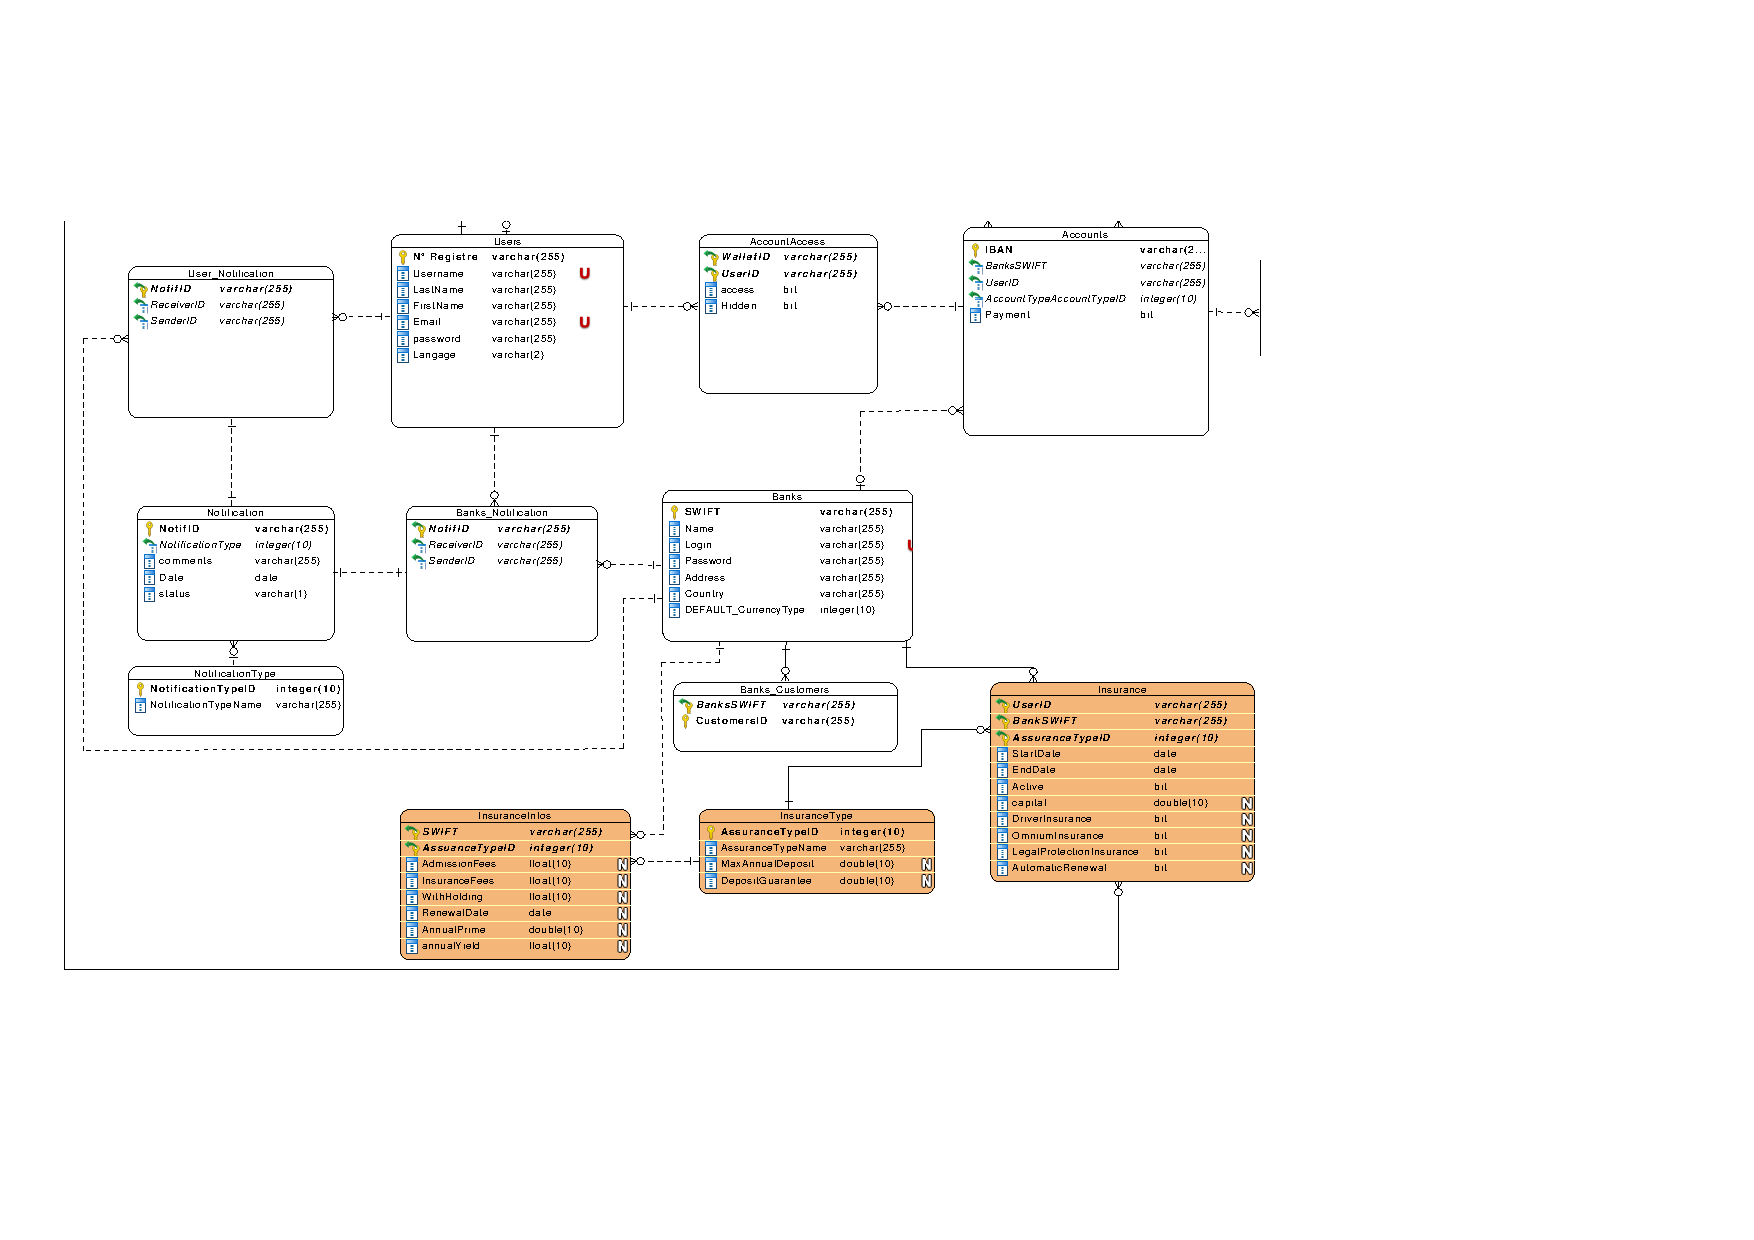
\includegraphics[scale=0.55]{img/BDDAssurance.pdf}
\caption{Diagramme d'entité-relation comprenant la partie assurance}
\label{fig1}
\end{figure}

\paragraph{}Pour la base de données, ses entités n’ont pas été modifiées mais cependant trois nouvelles ont été ajoutées. Globalement, il s’agit de données qui ne vont changer que rarement. Tout d’abord, l’entité Insurance contient les données qui dépendent du client comme le capital sur une assurance ou encore les option d’une assurance. Ensuite, l’entité InsuranceInfos reprend toutes les données d’une assurance qui dépendent de la banque comme le prix de l’assurance, le rendement pour les assurances vie, les différents frais ainsi que la date de renouvellement. Enfin, l’entité InsuranceType contient les données qui ne dépendent ni de la banque et ni du client comme le nom de l’assurance, le le dépot maximum ou la guarantie de dépot.

\end{document}